\documentclass[twocolumn]{aastex631}
\usepackage{mathtools}
\usepackage{natbib}
\bibliographystyle{abbrvnat}
\setcitestyle{authoryear,open={(},close={)}}
\usepackage{txfonts}
\usepackage{lipsum, babel}
\usepackage[T1]{fontenc}
\usepackage{ae,aecompl}
\usepackage{xcolor,colortbl}
\usepackage{tikz}
\usepackage{graphicx}
\usepackage{url}
\usepackage{floatrow}
%\usepackage[FIGTOPCAP]{subfigure}
\usepackage{subfigure}
\usepackage{float}
\usepackage{amsmath}
\usepackage{amssymb}
\usepackage{cleveref}
\usepackage{physics}
\usepackage{empheq}
\usepackage{booktabs}
\usepackage{array}
\newcolumntype{R}[1]{>{\raggedleft\arraybackslash}p{#1}}
\newcolumntype{L}[1]{>{\raggedright\arraybackslash}p{#1}}
\usepackage{multirow}
\usepackage[flushleft]{threeparttable}
\usepackage{mathrsfs}
\usepackage{soul}
\pdfminorversion=5

\newcommand{\MyDiamond}[1][fill=black]{
\begin{tikzpicture}[x=1.2ex,y=1.2ex,line width=.1ex,line join=round, yshift=0.0ex] \draw  [#1]  (0,.5) -- (.5,1) -- (1,.5) -- (.5,0);
\end{tikzpicture}
}

\newcommand{\MyPlus}[1][fill=black]
{
\begin{tikzpicture}[x=1.5ex,y=1.5ex,line width=0.5ex]
\draw[#1] (0,.5) -- (1,.5);
\draw[#1] (.5,0) -- (.5,1);
\end{tikzpicture}
}

\newcommand{\MyCross}[1][fill=black]
{
\begin{tikzpicture}[x=1.ex,y=1.ex,line width=0.5ex]
\draw[#1] (0,0) -- (1,1);
\draw[#1] (0,1) -- (1,0);
\end{tikzpicture}
}

\newcommand{\MyTriangle}[1][fill=black]
{
\begin{tikzpicture}[x=1.ex,y=1.ex,line width=0.2ex]
\draw[#1] (0,1) -- (1,1);
\draw[#1] (1,1) -- (.5,0);
\draw[#1] (.5,0) -- (0,1);
\fill[#1] (0,1) -- (1,1) -- (.5,0) -- cycle;
\end{tikzpicture}
}

\newcommand{\MySolidLine}[1][fill=black]
{
\begin{tikzpicture}[x=2.ex,y=1.ex,line width=0.5ex]
\draw[#1] (0,.5) -- (2.5,.5);
\end{tikzpicture}
}

\newcommand{\MyDashedLine}[1][fill=black]
{
\begin{tikzpicture}[x=2.ex,y=1.ex,line width=0.5ex]
\draw [#1,dashed] (0,.5) -- (2.5,.5);
\end{tikzpicture}
}

\newcommand{\MyDashedDottedLine}[1][fill=black]
{
\begin{tikzpicture}[x=2.ex,y=1.ex,line width=0.5ex]
\draw [#1,dash dot] (0,.5) -- (2.5,.5);
\end{tikzpicture}
}

\newcommand{\MyDottedLine}[1][fill=black]
{
\begin{tikzpicture}[x=2.ex,y=1.ex,line width=0.5ex]
\draw [#1,dotted] (0,.5) -- (2.5,.5);
\end{tikzpicture}
}

\definecolor{Gray}{gray}{0.85}

\begin{document}
\title{The symmetric \textit{Fermi} and eROSITA bubbles problem: A proof-of-concept study}


\author[0000-0002-1868-0660]{Po-Hsun Tseng}
\affiliation{Institute of Astrophysics, National Taiwan University, Taipei 10617, Taiwan}

\author[0000-0003-3269-4660]{H.-Y. Karen Yang}
\affiliation{Institute of Astronomy, National Tsing Hua University, Hsinchu 30013, Taiwan}
\affiliation{Center for Informatics and Computation in Astronomy, National Tsing Hua University, Hsinchu 30013, Taiwan}
\affiliation{Physics Division, National Center for Theoretical Sciences, Taipei 10617, Taiwan}

\author[0000-0002-1249-279X]{Hsi-Yu Schive}
\affiliation{Institute of Astrophysics, National Taiwan University, Taipei 10617, Taiwan}
\affiliation{Department of Physics, National Taiwan University, Taipei 10617, Taiwan}
\affiliation{Center for Theoretical Physics, National Taiwan University, Taipei 10617, Taiwan}
\affiliation{Physics Division, National Center for Theoretical Sciences, Taipei 10617, Taiwan}

\author{Chun-Yen Chen}
\affiliation{Institute of physics, National Taiwan University, Taipei 10617, Taiwan}

\author[0000-0003-2654-8763]{Tzihong Chiueh}
\affiliation{Institute of Astrophysics, National Taiwan University, Taipei 10617, Taiwan}
\affiliation{Department of Physics, National Taiwan University, Taipei 10617, Taiwan}
\affiliation{Center for Theoretical Physics, National Taiwan University, Taipei 10617, Taiwan}


\correspondingauthor{Po-Hsun Tseng}
\email{zengbs@gmail.com}


\keywords{keywords}

\begin{abstract}
\end{abstract}

\section{Introduction}
Over the last decade the discovery of the \textit{Fermi} bubbles \citep{Su2012,Ackermann2014,Narayanan2017},\
the high resolution X-ray map \citep{Predehl2020} from eROSITA \citep{Predehl2021} also shows\
similar X-ray bubbles above and below the Galaxy,\
but about twice as large as the Fermi bubbles, each having a diameter of about 45,000 lightyears.\

The \textit{Fermi} and eROSITA bubbles, two couple giant bubbles extending about 50 degrees\
above and below the Galactic center (GC),\
are among the most important findings of the Fermi Gamma-ray Space Telescope\

The Fermi bubbles and large-scale X-ray emission revealed by eROSITA\
show remarkable morphological similarity.

Early attempts to model the Fermi bubbles assumed that the jet is vertial to the Galactic plane...

\section{Methodology}

  We used the GPU-accelerated special relativistic hydrodynamics AMR code (\textsc{gamer-sr}) developed at the\
  National Taiwan University\
  (Schive et al. \citeyear{gamer-1}, \citeyear{gamer-2}; \citeauthor{tseng2021} \citeyear{tseng2021})\
  to carry out the simulations of the Fermi and eROSITA bubbles by CR and relativistic fluid injections from the GC.

  The CRs are advected with the thermal gas, and in return the velocities of gas\
  can react to the gradients of the CR pressure via the source term\
  containing spatial divergence of fluid velocities.\

  Although the high-energy CRe ($10$ --- $100$ GeV) plays a crucial role in reproducing the $\gamma$-ray map\
  within the range of $1$ --- $100$ GeV, we assume the pressure of CRe is much less than that of gas\
  throughout the simulation so that we , and the Fermi bubbles can be outlined against the eROSITA bubbles.

  As stressed by \citet{Yang2012}, CR diffusion has an insignificant effect on the overall morphology of the Fermi bubbles,\
  but only sharpens the edges of the simulated bubbles by the interplay between anisotropic CR diffusion\
  and magnetic fields with suppressed perpendicular diffusion across the bubble surface. Moreover,\
  the bubbles should be weak due to adiabatic expansion, and thus the magnetic fields has\
  a little effect on the overall dynamics. For these two reasons,\
  we have ignored the CR diffusion and the magnetic field throughout\
  the simulation.

  We do not simulate the spectral evolution of the CR, and we neglected the cooling and heating processes of CRs,\
  such as energy losses due to synchrotron and inverse Compton emission, and reacceleration in shocks.\

  In this approach, we treat CRs as a single species without distinction between electrons and protons,\
  that cannot react to the gas via the application of CRe pressure,\
  and solve directly for the evolution of CR energy density $e_{\text{cr}}$\
  as a function of $\mathbf{r}$ and $t$.\

  Since the relativistic fluid ejected by the jet source\
  is quickly stalled off and slowed down by a dense ISM disk in a short time,\
  and the relativistic fluid\
  accounts for a little minority of total mass inside the simulation box,\
  we still use the Newtonian gravity to attack this problem.

  The governing equations solving the special relativistic ideal fluid\
  including CR advection, and dynamical coupling between the thermal gas and CRs without CR diffusion\
  can be written a succinct form as


  \begin{subequations}
    \label{governing-eq}
    \begin{align}
     &\partial_{t} D+\partial_{j} \left(DU^{j}/\gamma\right)=0,\label{D evolution}\\
     &\partial_{t} M^{i}+\partial_{j} \left(M^{i}U^{j}/\gamma+p_{\text{gas}}\delta^{ij}\right)=\
     -\rho\partial_{i}\Phi,\label{M evolution}\\
     &\partial_{t} \tilde{E}+\partial_j \left[\left(\tilde{E}+p_{\text{gas}}\right)U^{j}/\gamma\right]=0, \label{E evoltion}\\
     &\partial_{t} \left(\gamma e_{\text{cr}}\right) + \partial_{j} \left(e_{\text{cr}}U^{j}\right)=\
     -p_{\text{cr}} \partial_{j} U^{j},\label{D evolution}
    \end{align}
  \end{subequations}


  where the five conserved quantities of gas $D$, $M^{i}$, and $\tilde{E}$ are the mass density,\
  the momentum densities, and the reduced energy density, respectively.\
  The reduced energy density is defined by subtracting the rest mass energy density of gas\
  from the total energy density of gas.\
  $\gamma$ and $U^{j}$ are the temporal and spatial component of four-velocity of gas.\
  $\rho$ is the gas density in the local rest frame defined by $D/\gamma$.\
  $p_{\text{gas}}$ is the gas pressure.\
  $p_{\text{cr}}$ and $e_{\text{cr}}$ are the CR pressure and CR energy density measured in the local rest frame.\
  $\Phi$ is the gravitation potential.\
  $c$ is the speed of light, and $\delta^{ij}$ is the Kronecker delta notation.\
  Throughout this paper, Latin indices run from 1 to 3, except when stated otherwise.\

  The set of \Cref{governing-eq} is closed by using the Taub-Mathews equation of state \citep{Taub,TM_EOS}\
  that approximates the exact EoS \citep{Synge} for ultra-relativistically\
  hot gases coexisting with non-relativistically cold gases.

  \textsc{gamer-sr} adopts a new algorithm \citep{tseng2021} to convert between\
  primitive ($\rho$, $U^{j}$, $p$) and conserved variables ($D$, $M^{j}$, $\tilde{E}$),\
  significantly reducing numerical error caused by catastrophic cancellations\
  that commonly occur within the regions with high Mach number flows. e.g., jet-ISM interaction zones.

  \textsc{gamer-sr} also adaptively and locally reduce the min-mod coefficient\
  \citep{tseng2021} within the failed patch group.\
  Doing so provides an elegant way to avoid the use of pressure/density floor,\
  being unnatural but widely used in almost publicly available codes.\

  \subsection{The Galactic and Disk Models}
  As a proof-of-concept study, we approximate conventionally axisymmetric stellar potential of Milky Way\
  by a plane-parallel potential that is symmetric about the mid-plane $z=0$\
  in a simulation box size of\
  $14\times14\times28$ kpc, slightly larger than the size of eROISTA bubbles.

  The plane-parallel potential is fixed throughout our simulations and given by
  \begin{equation}
    \Phi_{\text{total}}(z) = \Phi_{\text{bulge}}(z) + \Phi_{\text{halo}}(z),
  \end{equation}
  where
  \begin{equation}
    \Phi_{\text{bulge}}(z)=\
    2\sigma^2_{\text{bulge}}\
    \ln\cosh\left(z\sqrt{\frac{2\pi G\rho_{\text{bulge}}^{\text{peak}}}{\sigma^2_{\text{bulge}}}}\right)
  \end{equation}
  is the potential of an isothermal slab mainly contributed by stars around the Galactic bulge, and\
  $\Phi_{\text{halo}}(z)=v^2_{\text{halo}}\ln\left(z^2+d^2_{\text{h}}\right)$\
  is a plane-parallel dark logarithmic halo potential.

  With the help of the isothermal and hydrostatic equilibrium conditions,\
  and assuming the interfaces between isothermal disk and atmosphere are in thermal pressure equilibrium,\
  we can write the steady-state gaseous density distributions,\
  confined in the total potential, of the disk and the Galactic atmosphere as\
  \begin{subequations}
  \begin{align}
     \displaystyle \rho_{\text{isoDisk}}(z) = \rho_{\text{isoDisk}}^{\text{peak}}
     \exp\left[-\frac{\Phi_{\text{total}}(z)}{k_{B}T_{\text{isoDisk}}/m_{\text{p}}}\right]&\label{isothermal-disk-density}\\
     \text{, if $|z| < z_{0}$}& \nonumber \\
     \nonumber\\
     \displaystyle \rho_{\text{atmp}}(z) = \rho_{\text{atmp}}^{\text{peak}}
     \exp\left[-\frac{\Phi_{\text{total}}(z)}{k_{B}T_{\text{atmp}}/m_{\text{p}}}\right]&\label{isothermal-atmp-density}\\
     \text{, otherwise,}& \nonumber
  \end{align}
  \label{disk-atm-sys}
  \end{subequations}
  where $m_{\text{p}}$ is the proton mass,\
  $T_{\text{isoDisk}}$ and $T_{\text{atmp}}$ is the temperature of the isothermal disk and atmosphere,\
  $\rho_{\text{isoDisk}}^{\text{peak}}$ and $\rho_{\text{atmp}}^{\text{peak}}$ is the peak mass density\
  of the disk and atmosphere on the mid-plane $z=0$.

  We tabulate parameters in the first four\
  categories of \Cref{table-parameters},\
  except for $\rho_{\text{atmp}}^{\text{peak}}$ that\
  can be derived from the other known parameters and thermal pressure equilibrium condition\
  on the interfaces $(z=\pm z_{0})$ between the disk and atmosphere.\

  The density profile of \Cref{disk-atm-sys} is shown in \Cref{fig__initial-density-profile}.\
  Beyond the core radius ($\sim 2 \text{ kpc}$) the gaseous density decreases rapidly as a power-law.

%  The density profile of \Cref{disk-atm-sys} is shown in \Cref{fig__initial-density-profile}\
%  and compared to the observed result \citep{Miller_2013} beyond 1 kpc.\
%
%  Note that there is an difficulty in disentangling the contribution\
%  of the Local Bubble, a supernova remnant in which the Solar System is embedded \citep{Snowden1990},\
%  and the contribution from solar wind charge-exchange processes, which produce soft\
%  X-ray emission throughout the Solar System. As a result, the density profile of the Galactic halo remains unclear\
%  \citep{BlandHawthorn2016}.

  \begin{figure}
    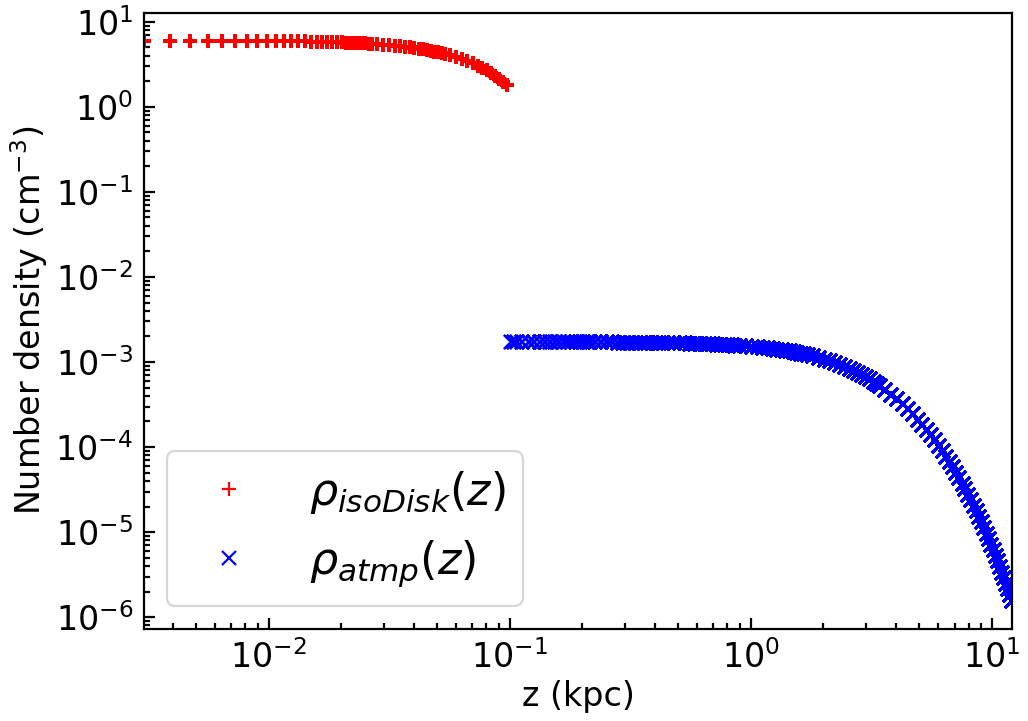
\includegraphics[width=\columnwidth]{figures/fig__initial-density-profile.png}
    \caption{The density profile of the isothermal disk (red pluses) and\
             atmosphere (blue crosses) along the positive z-axis.\
             The density distribution is derived from hydrostatic equilibrium,\
             the interface ($z=0.1$) between the isothermal disk\
             and the atmosphere is pressure balanced.}
    \label{fig__initial-density-profile}
  \end{figure}



  To quantify the synchrotron radiation as a function of position, it\
  is essential to start the simulation with a more realistic magnetic\
  field distribution. To this end, for our fixed magnetic field we adopt\
  the default exponential model in \textsc{galprop} \citep{Strong2007}
  which has the following spatial dependence:\

  \begin{equation}
     |\mathbf{B}(R, z)|=B_{0}\exp{-z/z_{0}}\exp{-R/R_{0}},
  \end{equation}


  where $R=\sqrt{x^{2}+y^{2}}$, $B_{0}$ is the average field strength at the GC\
  and $z_{0}$ and $R_{0}$ are the characteristic scales in the vertical and radial\
  directions, respectively. We adopt $z_{0} = 2$ kpc and $R_{0} = 10$ kpc, which\
  are best-fitting values in the \textsc{galprop} model to reproduce the\
  observed large-scale 408 MHz synchrotron radiation in the Galaxy.\
  We choose $B_{0} = 50$ $\mu$G based on the observed field strength at the\
  GC \citep{Crocker2010}.

   % The dispersion:
   %   2010-Comparing the statistics of interstellar turbulence in simulations and observations
   %   2011-RELATIVISTIC JET FEEDBACK IN EVOLVING GALAXIES


  \subsection{The Clumpy Multiphase Interstellar Medium}

  A crucial component in our work is the clumpy ISM disk initialized by\
  the publicly available pyFC code
  \footnote{\url{https://pypi.python.org/pypi/pyFC}}.\

  pyFC randomly generates dimensionless 3D scalar field $f(\bold{x})$\ % that is clumpy and porous.
  that obeys the log-normal probability distribution\
  with mean $\mu$ and dispersion $\sigma$,\
  and follows the power-law Kolmogorov spectrum
  \begin{equation}
    D(\bold{k})=\int k^{2} \hat{f}(\bold{k})\hat{f}^{*}(\bold{k})d\Omega \propto k^{-\beta},
    \label{Kolmogorov-spectrum}
  \end{equation}
  where $\hat{f}(\bold{k})$ is the Fourier transform of $f(\bold{x})$.\
  The spectrum $D(\bold{k})$ in the Fourier space is characterized by the power law index $\beta=5/3$,\
  the Nyquist limit $k_{\text{max}}$, and the lower cutoff wave number $k_{\text{min}}$.
  $k_{\text{max}}$ is one-half of the spatial resolution within disk,\
  and $k_{\text{min}}$ is 375.0, corresponding to the maximum size of an individual clump $\sim 20$ pc.\
  \citet{LA2002} and \citet{Wagner2012} have outlined a detailed procedure\
  for constructing a clumpy scalar field, and we do not repeat here.

  The density of clumpy disk can thus be obtained by taking the scalar products of\
  $f(\bold{x})$ with $\rho_{\text{isoDisk}}(z)$ over all cells within the disk, i.e.,\
  $\displaystyle\rho_{\text{ismDisk}}(\bold{x}) =\
  f(\bold{x}) \rho_{\text{isoDisk}}(z)$.\
  Also, the thermal pressure equilibrium within the clumpy disk implies that the temperature of disk is
  $\displaystyle T_{\text{ismDisk}}(\bold{x}) =\
  T_{\text{isoDisk}}(z)\rho_{\text{isoDisk}}(z)/\rho_{\text{ismDisk}}(\bold{x})$.


  \Cref{table-parameters} summarize the parameters of the clumpy disk and their references.

  On the basis of this setup, we cover the AMR base level with\
  $16\times16\times32$ root cells, refined progressively on the mid-plane $z=0$\
  based on the gradient of mass density.\
  We also restrict the refinement level at 7 within the cold disk so that\
  a molecular cloud can be adequately resolved by approximately 30 cells along their diameter, 20 pc.

  \Cref{fig__zoom-in-disk} shows a close-up view of the\
  pressure, temperature, and number density slices
  in the y-z plane through the center of the disk.

  \Cref{fig__numberDensityHistogram} plots the volume filling factor as a function of\
  initial number density within the disk without jet source.\

  \begin{figure}
      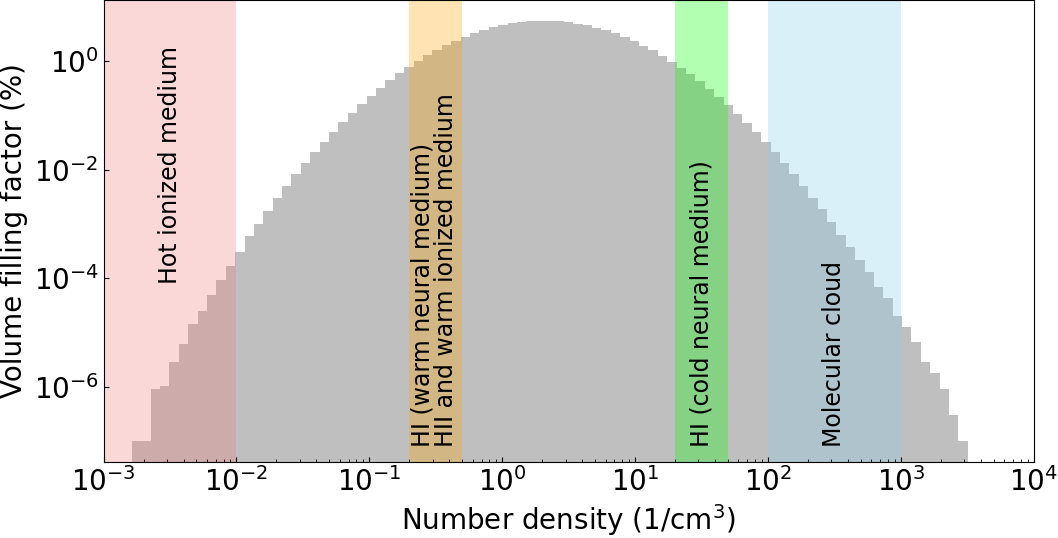
\includegraphics[width=\columnwidth]{figures/fig__numberDensityHistogram.png}
    \caption{The volume filling factor as a function of\
             initial number density within the disk without jet source.\
             The vertical bands represent from left to right: the allowable number densities \citep{peak-ism-density} for\
             hot ionized, warm neutral (WNM), warm ionized (WIM), cold nuetral mediums (CNM), and molecular clouds.}
      \label{fig__numberDensityHistogram}
  \end{figure}

  \begin{figure}
    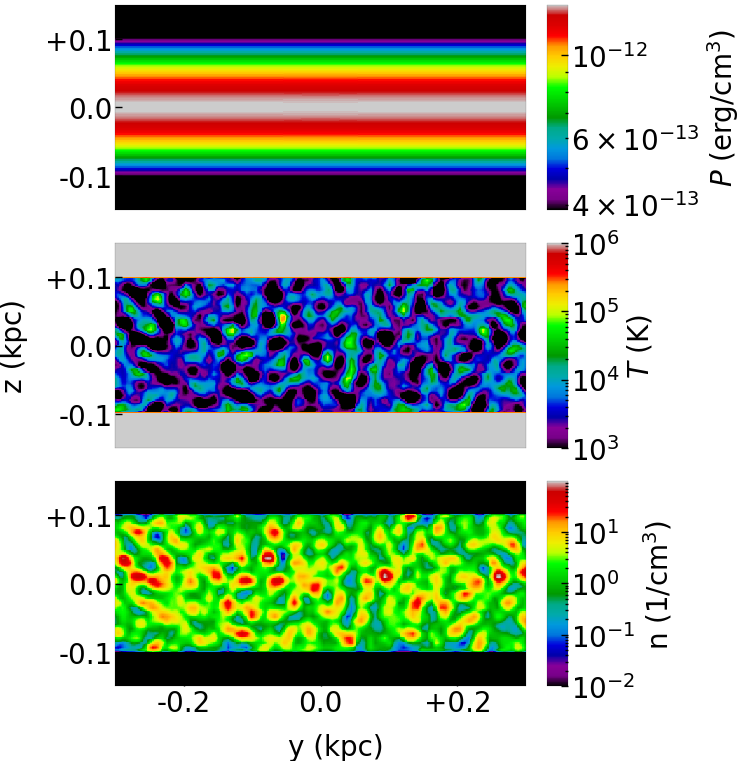
\includegraphics[width=\columnwidth]{figures/fig__zoom-in-disk.png}
    \caption{Close-up view of the initial\
             pressure (top), temperature (middle), and number density (bottom) slices\
             in the y-z plane through the center of the disk.
             }
    \label{fig__zoom-in-disk}
  \end{figure}

\begin{table*}[t]
\raggedright
\caption{Parameters of the disk, atmosphere, and gravitational potential in the simulation.}
\label{table-parameters}
\begin{tabular}{@{}llrc@{}}
\toprule[1pt]\midrule[0.3pt]
Parameter                             & Description                               & Value                                &  Reference                     \\ \midrule
{\bf Static stellar potential }       &                                           &                                      &                                \\
$\sigma_{\text{bulge}}$               & Velocity dispersion of bulge              & 100 km$\cdot$s$^{-1}$                & \citep{velocity-dispersion-MW} \\
$\rho_{\text{bulge}}^{\text{peak}}$   & Peak average density of bulge             & $4\times 10^{-24}$ g$\cdot$cm$^{-3}$ &   N/A                          \\ \hline
{\bf Static dark halo potential }     &                                           &                                      &                                \\
$v_{\text{halo}}$                     &                                           & 131.5 km$\cdot$s$^{-1}$              & \citep{Johnston1995}           \\
$d_{\text{h}}$                        & Core radius                               & 12 kpc                               & \multicolumn{1}{c}{''}         \\ \hline
{\bf Atmosphere }                     &                                           &                                      &                                \\
$T_{\text{\text{atmp}}}$              & Temperature of atmosphere                 & $10^{6}$ K                           & \citep{temperature-MW}         \\ \hline
{\bf Isothermal disk }                &                                           &                                      &                                \\
$z_{0}$                               & Scale height of disk                      & 100 pc                               & \citep{peak-ism-density}       \\
$T_{\text{\text{isoDisk}}}$           & Temperature of disk                       & $10^{3}$ K                           & \multicolumn{1}{c}{''}         \\
$\rho_{\text{isoDisk}}^{\text{peak}}$ & Peak mass density of disk                 & $10^{-23}$ g$\cdot$cm$^{-3}$         & \multicolumn{1}{c}{''}         \\ \hline
{\bf Clumpy disk }                    &                                           &                                      &                                \\
$\dagger$  $k_{\text{min}}$           & Cutoff wave number                        & 375.0                                & \citep{peak-ism-density}       \\
$\mu$                                 & Mean of scalar field                      & 1.0                                  &   N/A                          \\
$\ddag$  $\sigma$                     & Dispersion of scalar field                & 5.0                                  & \citep{Federrath2010}          \\
$\beta$                               & Power law index                           & -5/3                                 &   N/A                          \\ \midrule
\end{tabular}
\begin{tablenotes}
      \raggedright
      \item  $\dagger$  $k_{\text{min}}=375.0$ leads to the size of an individual molecular cloud $\sim 100$ pc.
      \item  $\ddag$ In numerical simulations of turbulence,\
             \citet{Federrath2010} find $\sigma\sim 3.6$ and 35 for solenoidal (divergence-free)\
             and compressive (curl-free) driving force,\
             respectively, so that our adopted value of 5 is closer to their solenoidal result.
    \end{tablenotes}
\end{table*}


% In addition to the gravitational interaction, we ignore other interactions between stars and gases.
% We also ignore the self-gravity of the ISM disk and of the atmosphere.
% We ignore the centrifugal force of Milky Way rotation acting on the bubbles.
%

\subsection{Inclined jet injection}
  Early observation \citep{Gallimore2006} has proposed that\
  there is a lack of preferred orientation of jets with respect to the plane of the disc.\
  A number of galaxies in which the jets are tilted to the disc normal\
  (e.g. NGC 3079, \citealt{Cecil2001}; NGC 1052, \citealt{Dopita2015}),\
  including galaxies in which the jets lie in the plane of the disc (e.g. IC 5063, \citealt{Morganti2015}).

  Motivated by these observations, we simulate the jet with an inclination angle\
  $45^{\circ}$ with respect to the Galactic plane\
  in order to release the caveat that\
  the jet direction must be perpendicular to the Galactic plane, and in particular to\
  investigate the effect of the jet-disk misalignment on the symmetry of bubbles.


  A few additional quantities are used to characterize the jets:
  the density contrast between the thermal gas contained in the jet source and the ambient gas,\
  $\rho_{\text{jet}}/\rho_{\text{amb}}=10^{-3}$,\
  the temperature contrast, $T_{\text{jet}}/T_{\text{amb}}=2\times10^{4}$,\
  the pressure ratio of CR to gas is 0.18,\
  and the flow 4-velocity inside the jet source $\beta\gamma = 0.6$\
  along the symmetric axis of cylinder.\
  The jet power is thus $3.2\times 10^{42}$ erg/s, resulting in the Eddington ratio 0.008.

  Note that as we inject the jets at the center of the clumpy disk,\
  we define the ambient gas density by the peak density of\
  the isothermal disk on the mid-plane $z=0$ (i.e. $\rho^{\text{peak}}_{\text{isoDisk}}$),\
  as opposed to the \textit{clumpy} density around the jet source, to avoid ambiguous definition.


  The bipolar jets are constantly ejected from a cylindrical source within a jet duration time 1.2 Myr,\
  allowing the total ejected energy $1.2\times10^{56}$ erg is between\
  $8\times10^{55}$ erg and $1.3\times10^{56}$ erg, estimated by \citet{Predehl2020}.\


  The diameter and height of cylindrical source are 4 pc, leading to the source volume $\sim 50 \text{ pc}^{3}$ is\
  much smaller than that of an individual clump by a factor of about 83.\
  By intentionally reducing the volume ratio of the jet source to an individual clump,\
  we can mitigate the effect of the randomness of the clumps on the bubbles.\
  Moreover, we resolve the jet source with the highest refinement level 11,\
  bringing the finest spatial resolution up to 0.4 pc.\



\section{Results}

  \begin{figure}
    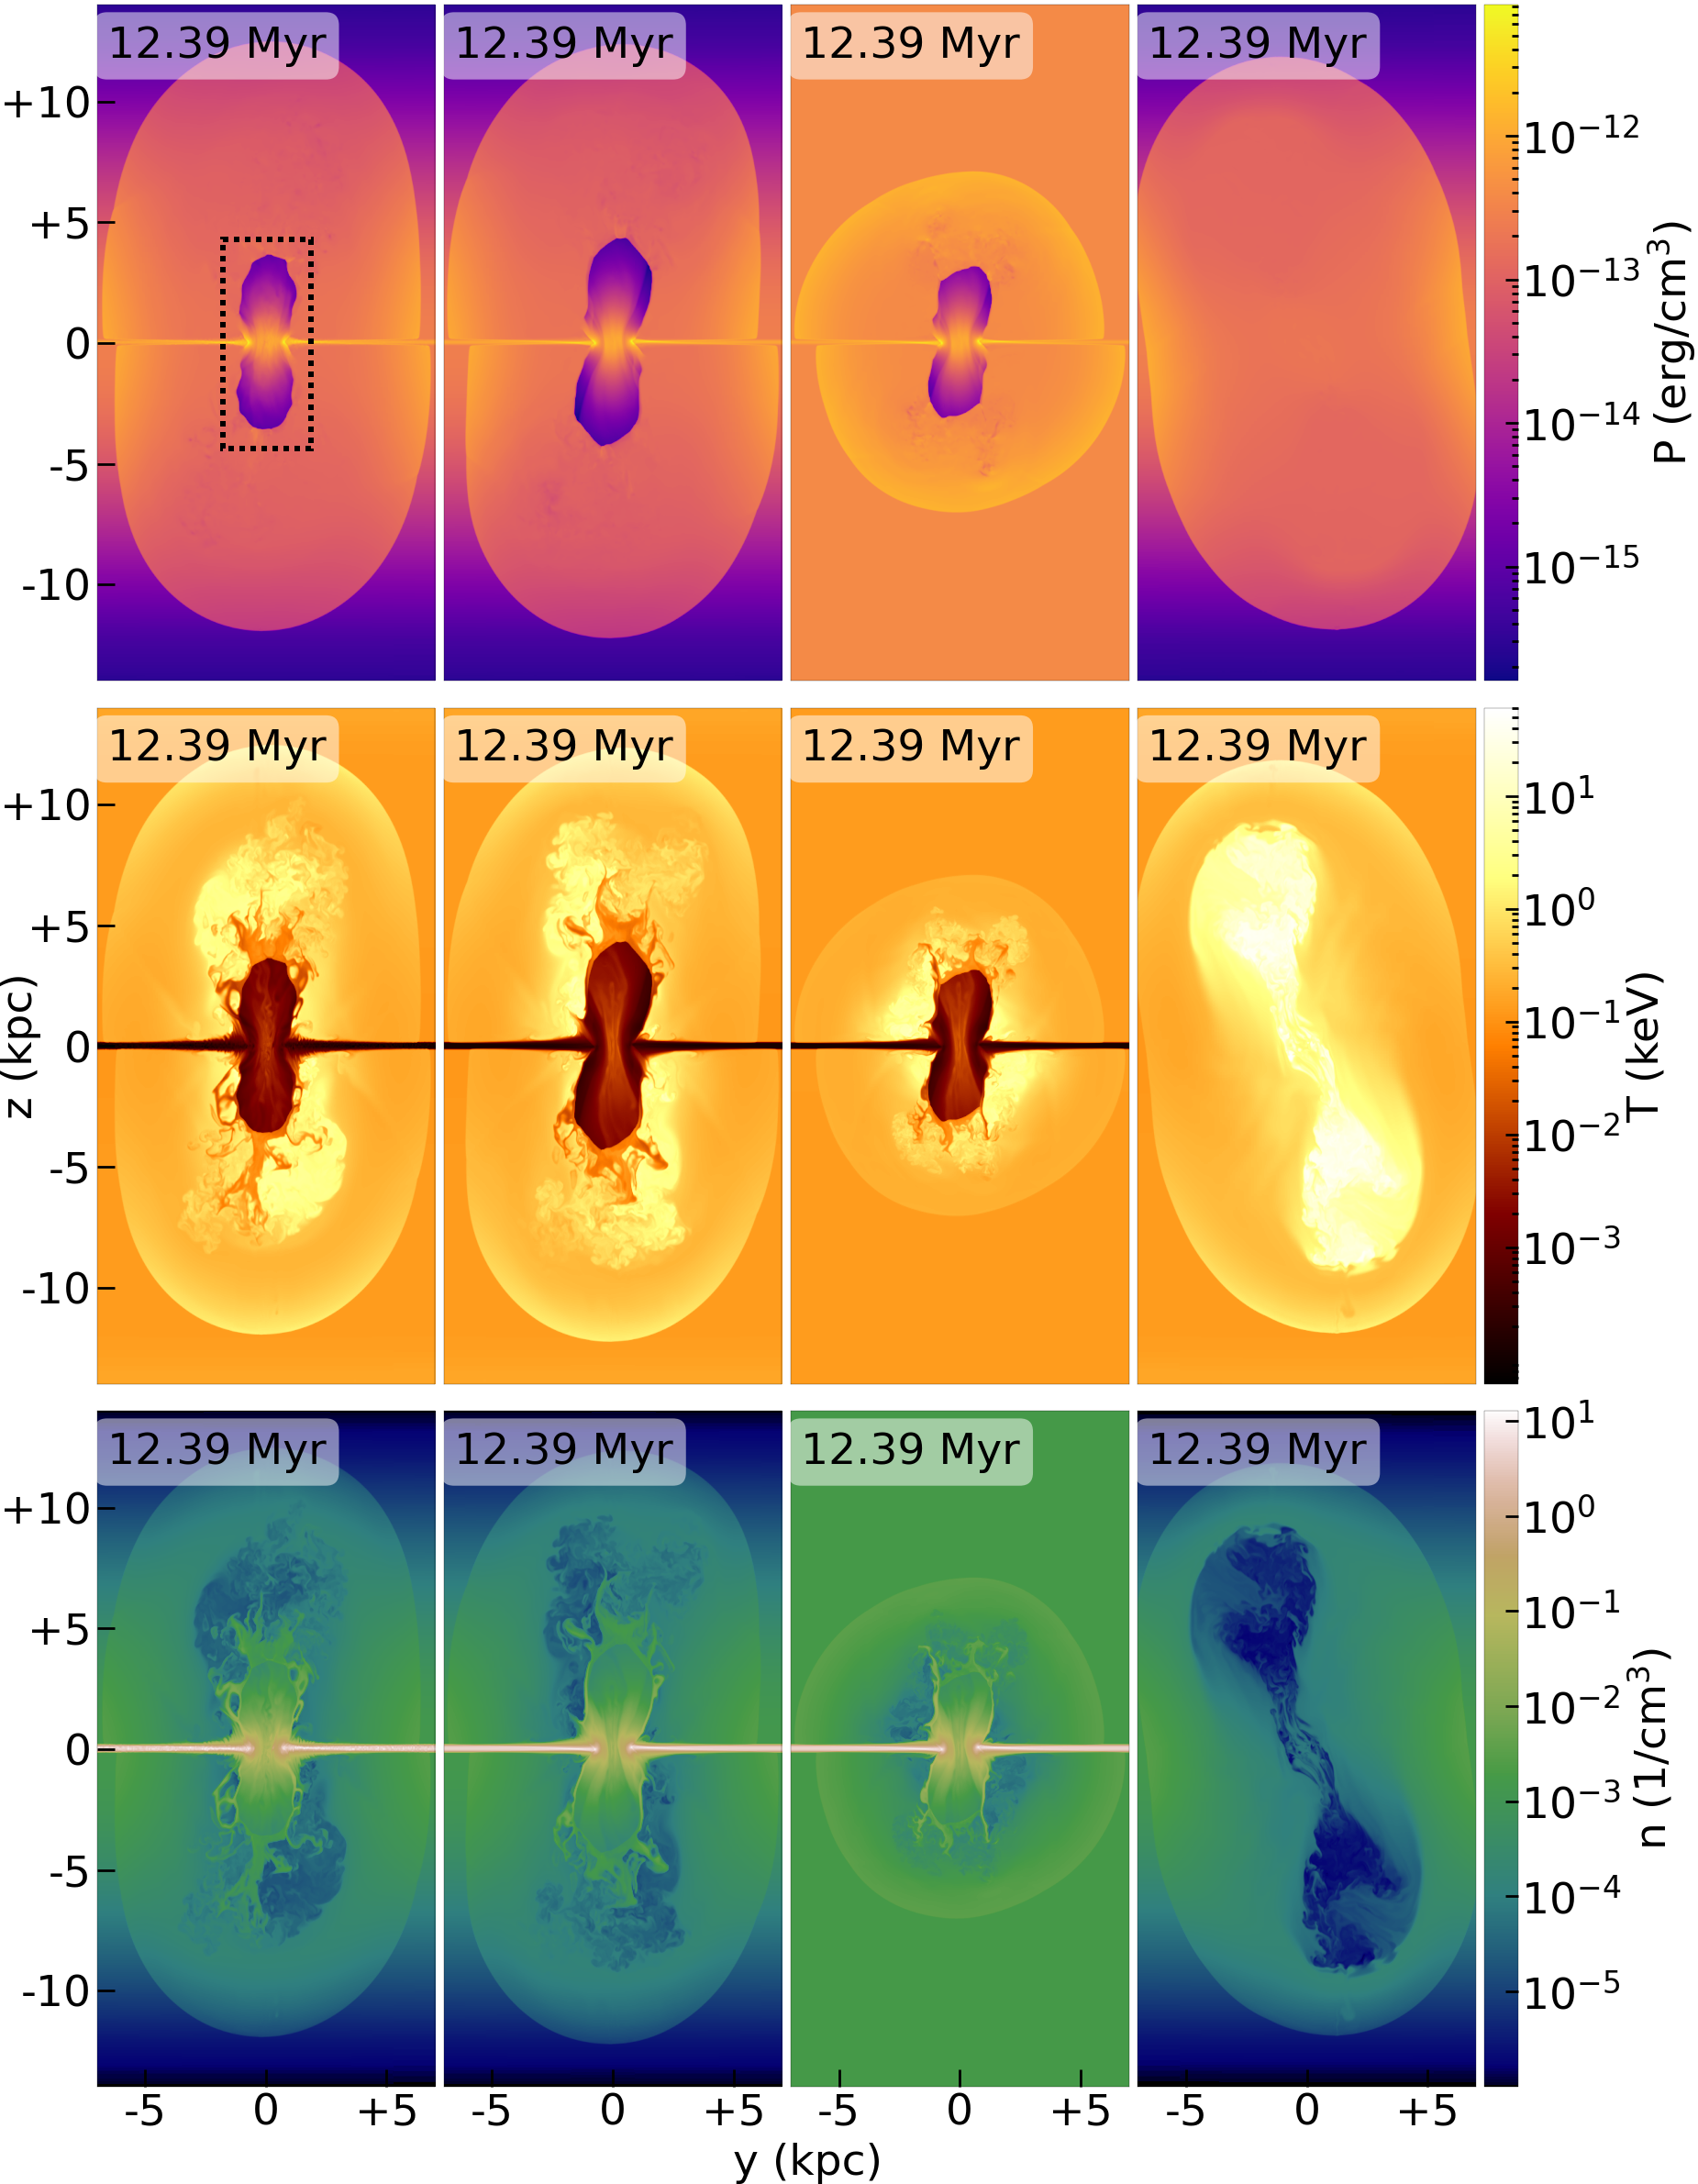
\includegraphics[width=\columnwidth]{figures/fig__jetI5+ismSeed3-45deg_no-disk-stratified-ambient-Pres-Dens-Temp.png}
    \caption{
             The pressure (top), temperature (middle), and number density (bottom) slices\
             through a bipolar jet sources injecting along $z=-y$ direction from\
             the origin for a duration of 1.2 Myr under four different cases from left to right.\
             Comparison between the cases with a clumpy (first column from left)\
             and with a smooth disk (second) in a stratified atmosphere\
             shows that the initial density distribution of the dense disk has an insignificant effect\
             on the overall dynamics of bubbles. However, the outer bubbles with the smooth disk\
             in an uniform atmosphere (third) is spherical-shape,\
             suggesting the stratification facilitates the outer bubbles elongation significantly.\
             Also, the first three and the rightmost columns show that the most inner bubbles (dashed box)\
             can only appear associated with the disk, and without the disk, the outer bubbles will be tilted,
             indicating the dense disk is crucial for\
             the axis-symmetrically outer bubbles and of the most inner bubbles formation.
             }
    \label{fig__jetI5+ismSeed3-45deg_no-disk-stratified-ambient-Pres-Dens-Temp}
  \end{figure}


\subsection{X-ray emission}


Thermal bremsstrahlung: The X-ray emissivity in an energy range 1.4–1.6 keV is calculated\
using the MEKAL model \citep{Xray-1,Xray-2,Xray-3}\
implemented in the utility XSPEC \citep{XSPEC}, assuming solar metallicity.\

Note that the observed X-ray emission is contributed by all the gas in the Milky Way halo,\
which likely extends to a radius of $\sim$250 kpc \citep{halo-radius-1,halo-radius-2},\
much bigger than our simulation box. Therefore, we first compute the X-ray emissivity\
from the simulated gas within a radius of 25 kpc away from the GC.
Then, beyond 25 kpc the gas is assumed to be isothermal with $T=10^6$ K and\
follows out to a radius of 250 kpc the observed density profile of \citep{temperature-MW}.


  \begin{figure*}
    \subfigure[Simulated (top) and observed (bottom; \citealt{Predehl2020}) count rate\
               (photons s$^{-1}$ deg$^{-2}$) in the 0.6-1.0 keV range,\
               using a Hammer-Aitoff projection. Throughout this paper we show sky maps\
               in Galactic coordinates centered on the Galactic center and observed by the solar position.\
               The red arrow at the center of the\
               top panel depicts the direction of the bipolar jet, constantly ejecting at an angle of $45^{\circ}$\
               to the disk normal in 1.2 Myr.]
     {
      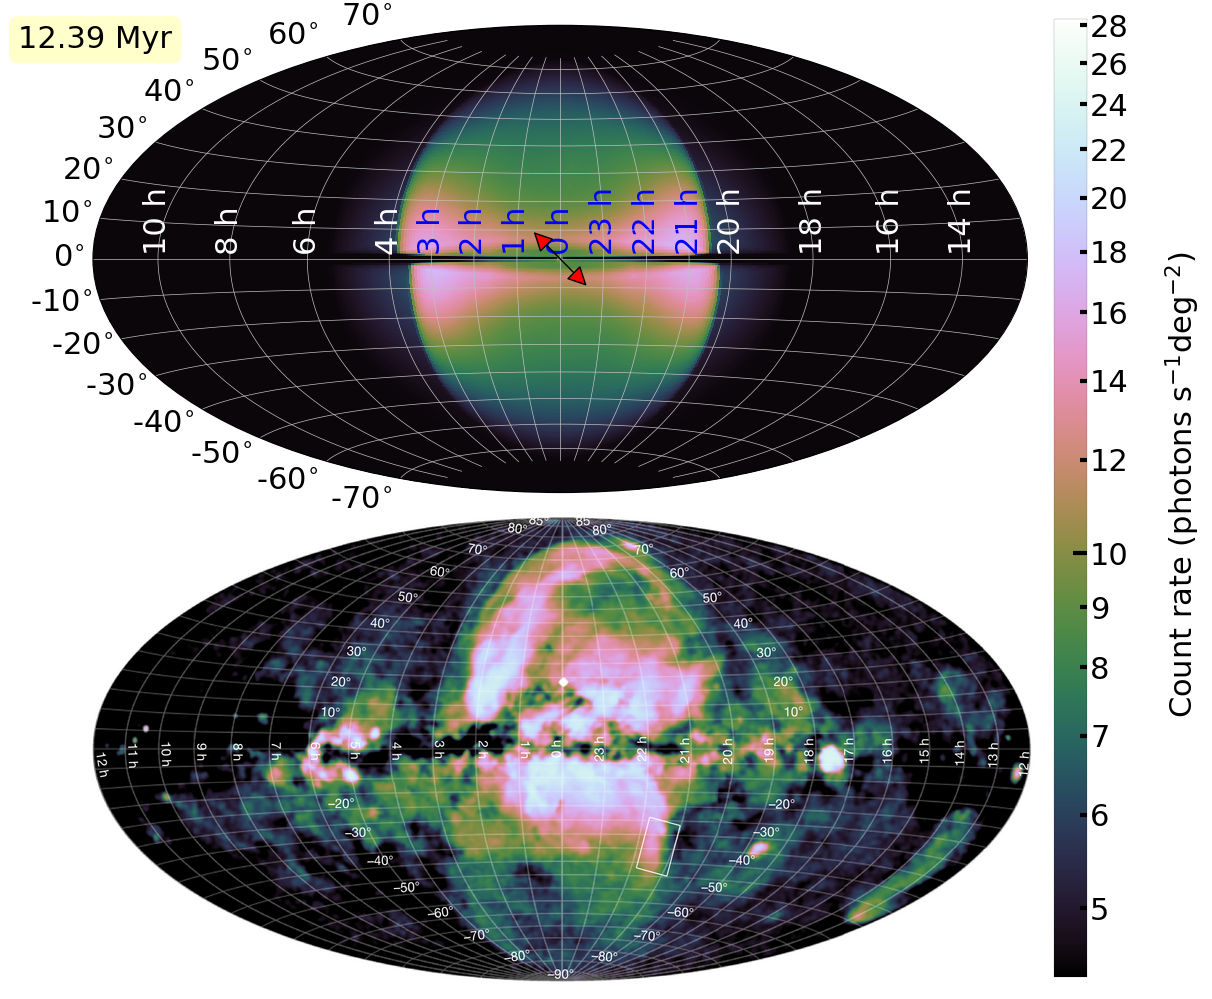
\includegraphics[width=0.8\linewidth]{figures/fig__xraymap.png}
      \label{fig__xray_0.8keV_angle_000}
     }
    \subfigure[Comparison of simulated (red) and observed (black; \citealt{Predehl2020}) one-dimensional\
               count rate profiles in the same energy band as \Cref{fig__xray_0.8keV_angle_000},\
               cut at various galactic latitudes (as labelled).]
     {
      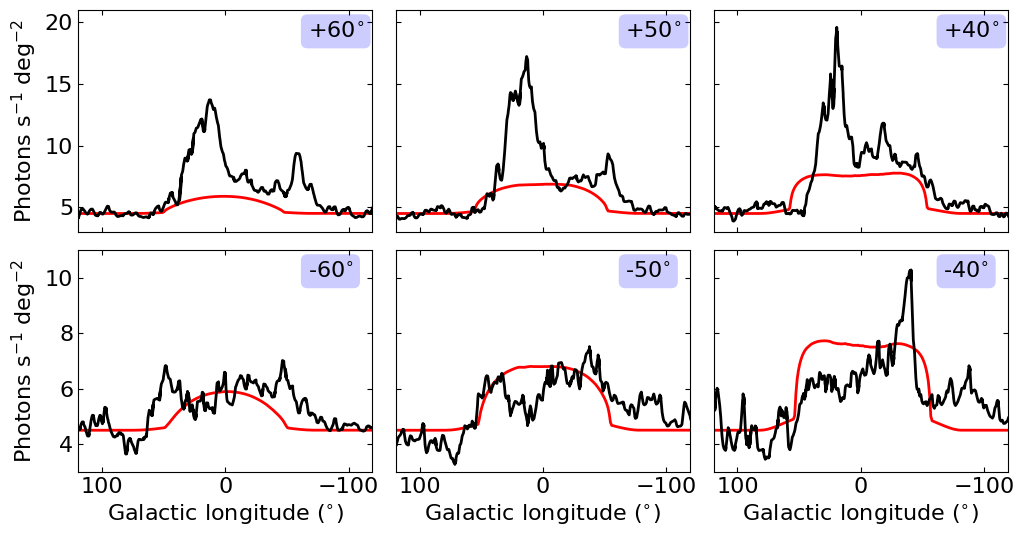
\includegraphics[width=0.8\linewidth]{figures/fig__xray-profile-0.8keV-000.png}
      \label{fig__x-ray-profile-0.8keV-000}
     }
    \caption{}
    \label{fig_xray}
  \end{figure*}

\subsection{Gamma-ray emission}

  \begin{figure}
    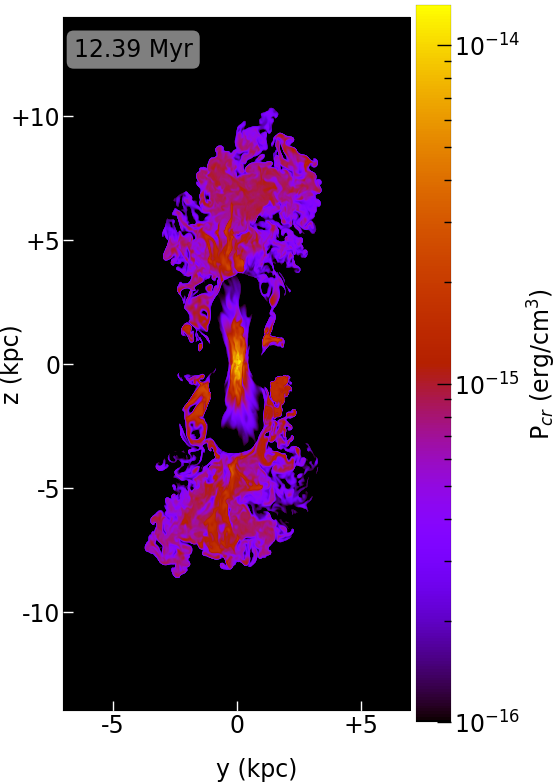
\includegraphics[width=\columnwidth]{figures/fig__jetI5+ismSeed3-45deg-CR.png}
    \caption{The slice of CR...}
    \label{fig__jetI5+ismSeed3-45deg-CR}
  \end{figure}

\subsubsection{Leptonic process}
In the leptonic scenario, the gamma-rays originate from IC scattering of the ISRF by CRe.\
The CRe spectrum follows a power law distribution\
with a spectral index $p=2.4$ and ranges from\
$m_{\text{e}}c^2$ ($0.5$ MeV) to $1.1\times10^{6}m_{\text{e}}c^2$ ($550$ GeV).\


The emissivity of the upscattered photons at the energy $\epsilon_{1}$ is given by\
the double integrals \citep{BLUMENTHAL1970}\
over the range of incident photon energy and the CRe Lorentz factor:

\begin{subequations}
  \begin{align}
  &\frac{dE}{dtd\epsilon_{1}dV} =\nonumber\\
               &\frac{3}{4}\sigma_{T}c\mathbb{C}\epsilon_{1}\int^{\epsilon_{\text{max}}}_{\epsilon_{\text{min}}}
               \frac{n(\epsilon)}{\epsilon}d\epsilon\int^{\gamma_{\text{max}}}_{\gamma_{\text{min}}\left(\epsilon\right)}
               \gamma^{-(p+2)}f(q, \Gamma)d\gamma,\\
  \nonumber\\
  &f(q, \Gamma) =\nonumber\\
               &2q\ln q+(1+2q)(1-q)+0.5(1-q)\frac{\left(\Gamma q\right)^2}{1+\Gamma q},\\
  &q=\frac{\epsilon_{1}/\gamma\
               m_{\text{e}}c^{2}}{\Gamma\left(1-\epsilon_{1}/\gamma m_{\text{e}}c^{2}\right)},\\
  &\Gamma=\frac{4\epsilon \gamma}{m_{\text{e}}c^2},\\
  &\gamma_{\text{min}}(\epsilon)=\
   0.5\left(\frac{\epsilon_{1}}{m_{\text{e}}c^2}+\sqrt{\left(\frac{\epsilon_{1}}{m_{\text{e}}c^2}\right)^2+\
   \frac{\epsilon_{1}}{\epsilon}}\right),
  \end{align}
\end{subequations}

where $\sigma_{T}$ is the Thomson cross section, $c$ speed of light, $m_{\text{e}}$ electron mass,\
$n(\epsilon)$ the photon number density of ISRF per energy, $\gamma$ the Lorentz factor of CRe,\
$\mathbb{C}$ and $p$ are the normalization constant and spectral index of CRe power-law spectrum,\
$\gamma_{\text{min}}(\epsilon)$ is the minimum required Lorentz factor of CRe such that CRe is energetic sufficient for\
producing scattered photon at the energy $\epsilon_{1}$ from an incident photon energy $\epsilon$.\
$\gamma_{\text{max}}$ is the maximum CRe Lorentz factor in the spectrum, i.e. $\gamma_{\text{max}}=10^{6}$.


We integrate the incident photon energy from\
$\epsilon_{\text{min}}=1.13\times10^{-4}$ eV (CMB radiation) to\
$\epsilon_{\text{max}}=13.59$ eV (starlight) in order to\
facilitate a reliable interpretation of simulated gamma-ray map.


The gamma-ray emissivity\
is computed for each computational cell in our simulations\
using the Klein–Nishina IC cross-section \citep{Jones1968} based\
on the simulated CR number density and the ISRF model given by \citet{Porter2017}.


To evaluate the simulated photon flux $I$ at the energy $\epsilon_{1}$ and\
take into account the perspective projection effect,
we integrate the emissivity over line-of-sights from the solar position at $(x,y,z)=(8,0,0)$ kpc:
\begin{equation}
I = \frac{1}{\epsilon_{1}}\int \frac{dE}{dtd\epsilon_{1}dV} dl.
\end{equation}


\begin{figure*}
  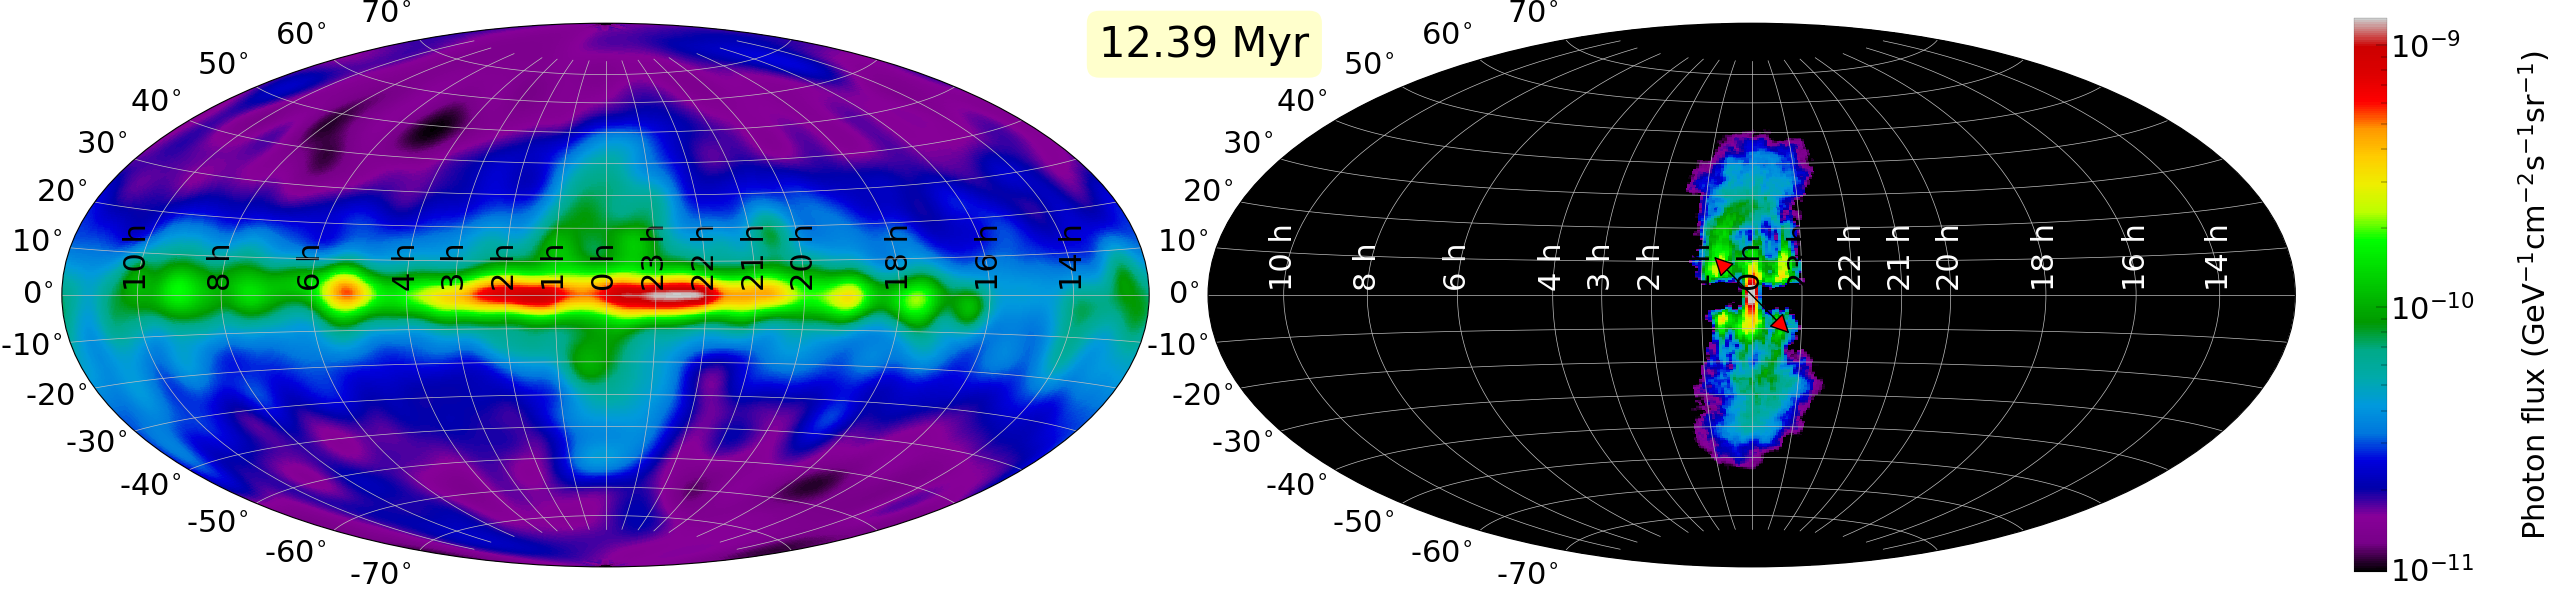
\includegraphics[width=\linewidth]{figures/fig__GammaRay_100e9_1e6_angle_000.png}
  \caption{The observed (left) and simulated (right) photon flux at 108.6 GeV.\
           Note that the left panel is the\
           photon flux of the diffuse component reconstructed by the D$^3$PO\
           algorithm \citep{Selig2015} that analyzes\
           the photon data from the \textit{Fermi} Large Area Telescope \citep{Atwood2009}\
           and removes the contribution from point-like component.
  }
  \label{fig__gammaRay}
\end{figure*}

\begin{figure*}
  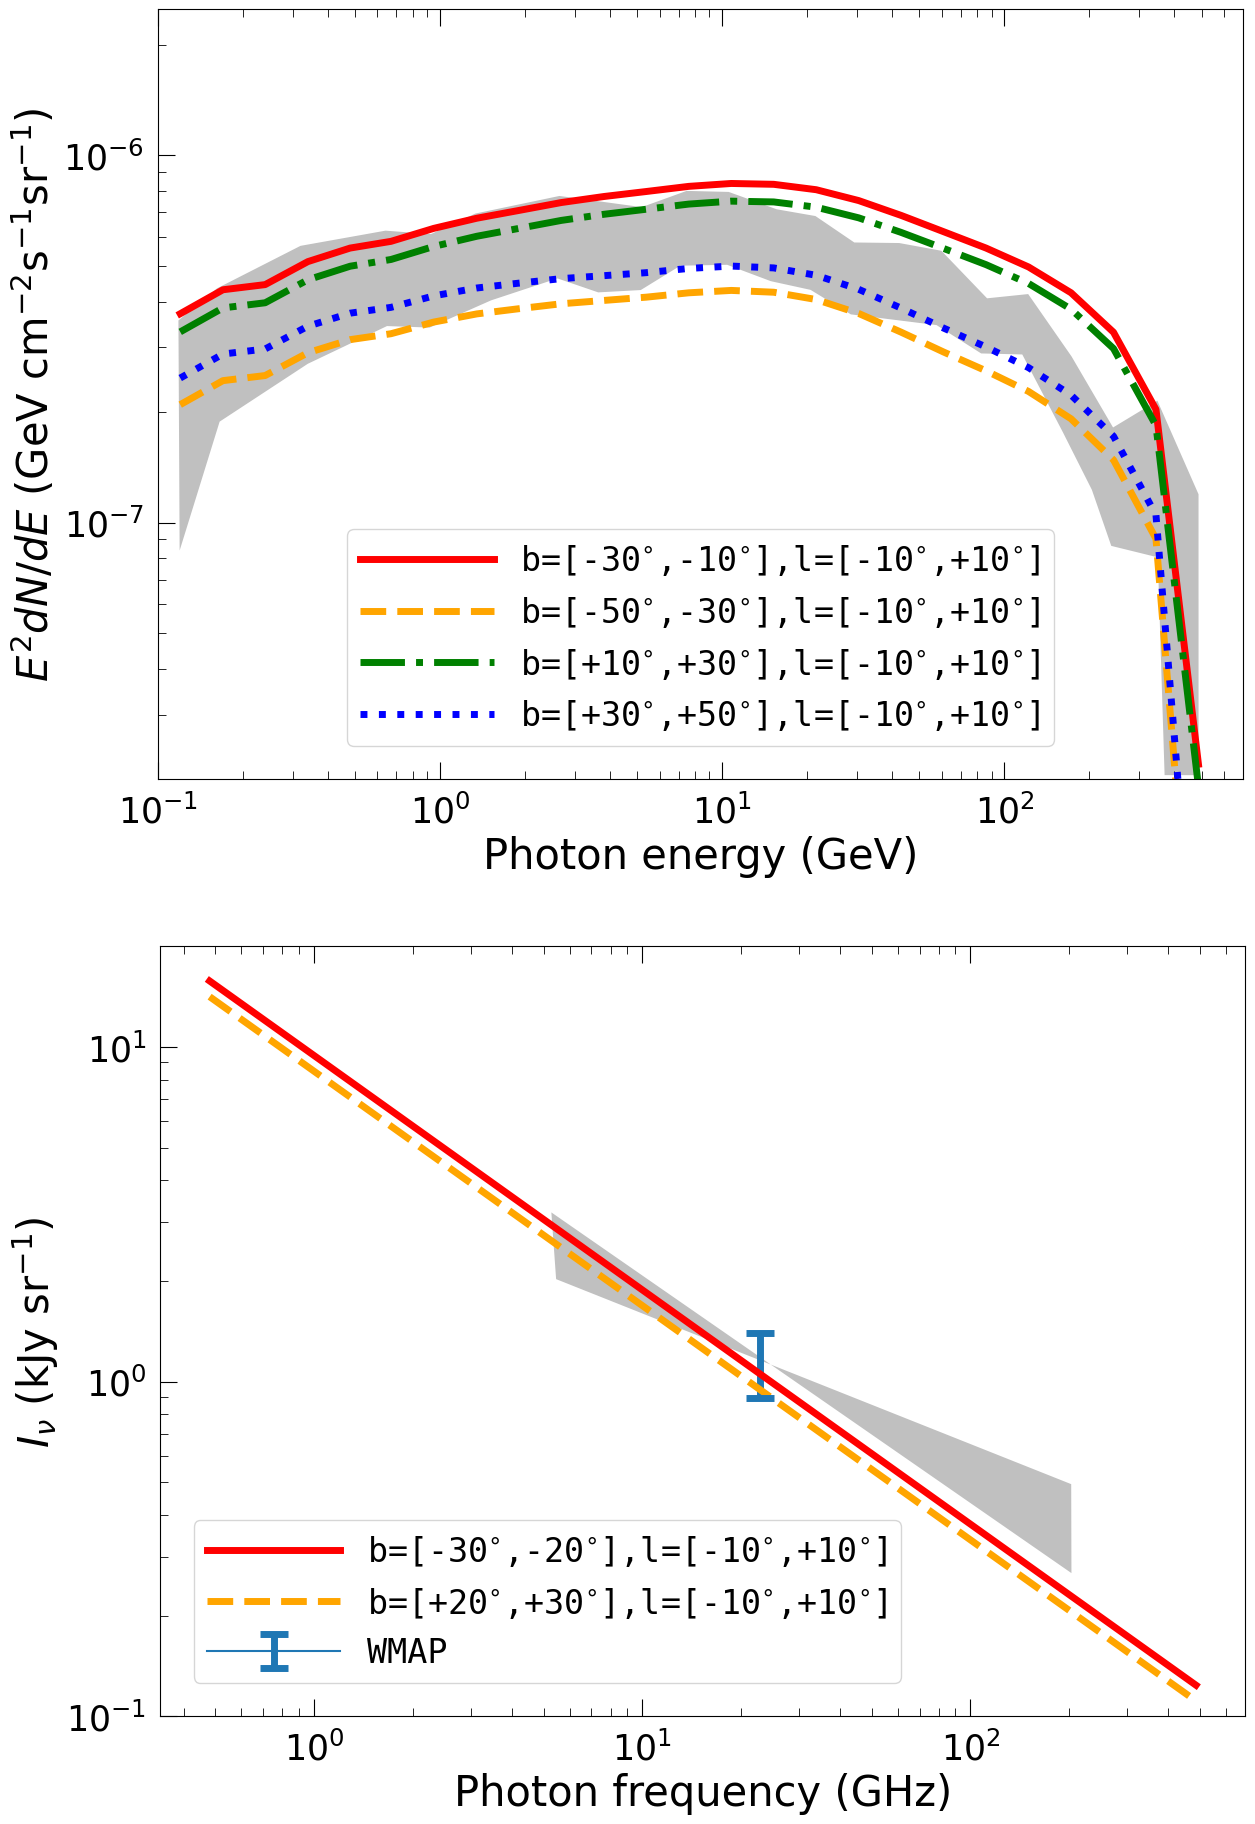
\includegraphics[width=\linewidth]{figures/fig__spectrum.png}
  \caption{
      Simulated gamma-ray spectra (colored lines in right column) of the Fermi bubbles calculated for a longitude range of\
      $|l|<10^{\circ}$ for different latitude bins.\
      The gray band represents the observational data of \citet{Ackermann2014}.\
      Simulated microwave spectra (colored lines in left) averaged over $|l|<10^{\circ}$, $20^{\circ}<|b|<30^{\circ}$.\
      The data point represents the \textit{WMAP} data in the 23 GHz K band and the shaded area indicates the range\
      of synchrotron spectral indices allowed for the \textit{WMAP} haze \citep{Dobler_2008}.
  }
  \label{fig__gammaRay}
\end{figure*}

%\subsubsection{Hadronic process}
%In the hadronic model, CRp undergo hadronic collisions with thermal gas protons\
%and produce $\gamma$-ray via pion decay. The volume emissivity of the emission can be written as
%\begin{equation}
%   \epsilon \propto U_{\text{CRp}}n_{p}\sigma_{p}\kappa_{pp}.
%\end{equation}
%
%\begin{equation}
%  \frac{dE}{dtd\epsilon_{1}dV} =\
%   cn_{H}pC\left(\frac{\epsilon_{1}}{m_{\text{p}}c^2}\right)^{-p}\
%   \int_{0}^{1}\sigma(\epsilon_{\text{p}}) F(x,\epsilon_{\text{p}}) x^{p}dx.
%\end{equation}
%
%\begin{equation}
%\sigma(\epsilon_{\text{p}})=34.3+1.88L+0.25L^{2}\left[1-\frac{E_{\text{threshold}}}{E_{\text{p}}}\right]^{4} \text{ mb}.
%\end{equation}
%
%\begin{equation}
%F(x,\epsilon_{\text{p}})=B\frac{d}{dx}\left[\ln(x)\left(\frac{1-x^{\beta}}{1+kx^{\beta}\left(1-x^{\beta}\right)}\right)^4\right],
%\end{equation}
%
%
%where
%$x=\epsilon_{1}/\epsilon_{\text{p}}$, $B=1.30+0.14L+0.011L^2$, $\beta=\left(1.79+0.11L+0.008L^{2}\right)^{-1}$,\
%$\left(0.801+0.049L+0.014L^{2}\right)^{-1}$, $L=\ln(\epsilon_{\text{p}}/1 \text{ TeV})$.



\section{conclusions}

\section*{Data Availability}
The data underlying this article are available in the article and in its online supplementary material.


%%%%%%%%%%%%%%%%%%%% REFERENCES %%%%%%%%%%%%%%%%%%
\bibliographystyle{mnras}
\bibliography{paper} % if your bibtex file is called example.bib

%%%%%%%%%%%%%%%%% APPENDICES %%%%%%%%%%%%%%%%%%%%%

%\appendix
% https://heasarc.gsfc.nasa.gov/docs/objects/heapow/archive/normal_galaxies/fermibubbles_erosita.html

%Jet_SrcVel 0.6
%Jet_SrcDens 1e-26
%Jet_SrcTemp 2e10
%Jet_SrcPres => 1.6e-8

\end{document}
